\documentclass[../piano_di_progetto.tex]{subfiles}

\begin{document}


\subsection{Modello incrementale}
\label{sub:incr}

Per garantire la qualità del prodotto e uno sviluppo corretto che risulterà conforme rispetto ai requisiti richiesti sul lungo periodo, il gruppo ha scelto l’\glossario{approccio
incrementale}, ovvero l’impiego di \glossario{rilasci} che mirano ad integrare nel sistema ogni volta una nuova funzionalità. Questo sistema permette di ridurre il rischio di fallimento ad ogni iterazione, producendo un nuovo valore.

Il modello di sviluppo incrementale permette di progredire tramite cicli di incremento, 
ripetuti fino a quando il prodotto non soddisferà i requisiti richiesti dal cliente. \\
Il ciclo di incremento risulta suddiviso nei seguenti passi:
\begin{enumerate}
    \item Pianificazione;
    \item Analisi dei requisiti;
    \item Progettazione;
    \item Implementazione;
    \item Test;
    \item Valutazione.
\end{enumerate}
Ogni ciclo di incremento permette lo sviluppo di una funzionalità aggiuntiva.
La priorità nell'implementazione viene data alle funzionalità con importanza maggiore, quindi tutte quelle funzionalità base richieste dal committente o le funzionalità che sono dipendenze di altre. 
Seguendo questo modello le funzionalità principali e più importanti vengono implementate per prime, inserendo in questo modo quelle meno significative in un sistema stabile. 
La ciclicità prevista dal modello incrementale facilita anche il versionamento del sistema,
tracciando modifiche nette al software.\\
L'iter che verrà seguito dal gruppo per ogni fase è il seguente:
\begin{itemize}
    \item Il gruppo fissa degli incrementi e le relative date di scadenze entro le quali l'incremento deve essere concluso.
    \item Il carico di lavoro viene suddiviso tra i membri del gruppo in base ai ruoli assegnati.
    \item Al termine dell'incremento verrà analizzato il lavoro svolto e se gli obbiettivi sono stati rispettati (fase di \emph{verifica}).
\end{itemize}

\begin{figure}[H]
    \centering
    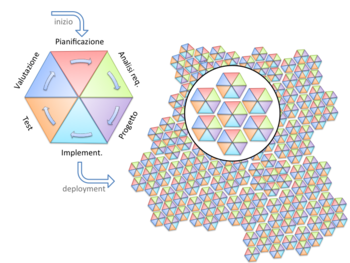
\includegraphics[scale = 0.6]{src/img/modello_incrementale.png}
    \caption{Rappresentazione del modello incrementale}
    \label{fig:logo}
\end{figure}

L'utilizzo di questo modello permette di ottenere importanti vantaggi, quali:
\begin{itemize}
    \item Maggior priorità alle funzionalità primarie, in questo modo possono essere sottoposte al cliente nel minor tempo possibile;
    \item Utilizzo dello sviluppo per incrementi successivi limita la modifica e le correzioni degli errori al singolo incremento, risultano meno onerose in termini di tempo e, di conseguenza, di costi;
    \item Le verifiche e i test sono circoscritti al singolo incremento, cioè alle nuove funzionalità;
    \item Possibilità di un maggior numero di feedback da parte del cliente, aumentando l'efficienza.
\end{itemize}


\subsubsection{Incrementi individuati}
\label{ssub:incr_ind}

Di seguito viene riportato un tracciato incremento | requisito, in modo tale da comprendere più chiaramente i requisiti che verranno soddisfatti in ciascun incremento. 
Gli UC o i requisiti verranno sviluppati all'interno dell'incremento associato ad essi e verranno considerati soddisfatti in tutti gli incrementi successivi a quello di sviluppo.




\subsubsection*{Progettazione e codifica della technology baseline}
\begin{table}[!ht]
	\centering
	\begin{tabular}{|p{3cm}|p{6.5cm}|}
	\hline
	\rowcolor{lightgray}
    \textbf{Incremento} & \textbf{Requisito}\\
    \hline
        Incremento I & RVO3\\
        Incremento II & RVO1\\
        Incremento III & UCW1.2  UCW3 \\
        Incremento IV & UCW2.2 UCW4.2.1 UCW4.2.2 UCW4.2.4 UCW4.2.5\\
        Incremento V & UCW1.3\\
    \hline
    \end{tabular}
    \caption{Tabella tracciamento incremento-obiettivi}
\end{table}

\newpage

\subsubsection*{Progettazione e codifica di dettaglio}

\begin{table*}[!h]
	\centering
	\begin{tabular}{|p{3cm}|p{6.5cm}|}
	\hline
	\rowcolor{lightgray}
    \textbf{Incremento} & \textbf{Requisito}\\
    \hline
        Incremento I & RFO01 \\
        Incremento II & RFO1.1, RF01.2 \\
        Incremento III & RFD4.3.1.1, RFD4.3.1.2, RFD4.3.1.4 \\
        Incremento IV & RFO2, RFO2.1, RFO2.2, RFD4.2, RFD4.2.2 \\
        Incremento V & RFO3, RFO3.1, RFO3.2, RFD4, RFD4.1 \\	
        Incremento VI &  RFO5, RFO6, RFO8 \\
        Incremento VII & RFO2.6, RFO4.5.2, RFO4.5.3.2, RFD4.7.5.6, RFD4.5, RFD4.5.1, RFD4.3.1, RFD4.5.6, RFF4.5.5, RFO4.5.3.1 \\
        Incremento VIII & RFO1.3, RFO1.3.1, RFO1.3.2, RFO7 \\
        Incremento IX & RFD4.2.3, RFD4.5.1.1, RFD4.5.1.2, RFD4.5.1.3 \\
        Incremento X & RFD4.2.4, RFD4.2.5, RFD4.8 \\
        Incremento XI & RFO3.3, RFD4.2.1, RFD4.3, RFD4.3.2.2, RFD4.3.2.3, RFD4.3.3 \\
        Incremento XII & RFO2.3 \\
        Incremento XIII & RFO2.5 \\
        Incremento XIV & RFO2.4, RFD4.7, RFD4.7.1, RFD4.7.1.1, RFD4.7.1.2, RFD4.7.1.3, RFD4.7.2, RFD4.7.3, RFD4.7.4, RFD4.7.5 \\        
    \hline	
	\end{tabular}
	\caption{Tabella tracciamento incremento-obiettivi}
\end{table*}

\subsubsection*{Validazione e collaudo}
\begin{table}[!h]
	\centering
	\begin{tabular}{|p{3cm}|p{6.5cm}|}
	\hline
	\rowcolor{lightgray}
    \textbf{Incremento} & \textbf{Requisito}\\
    \hline
        Incremento XV & RFD4.2.4, RFD4.2.5, RFD4.8 \\
        Incremento XVI & RFD4.4, RFD4.7, RFD4.7.1, RFD4.7.1.1, RFD4.7.1.2, RFD4.7.1.3, RFD4.7.2, RFD4.7.3 \\
        Incremento XVII & RFD4.4.2, RFD4.4.2.2, RFD4.4.1, RFD4.4.2.1, RFD4.4.2.3, RFD4.4.3.4, RFD4.4.5 \\
        Incremento XVIII & RFD4.7.1.3, RFD4.7.2, RFD4.7.3, RFD4.7.4, RFD4.7.5, RFD4.7, RFD4.7.1.1, RFD4.7.1.2 \\
        Incremento XIX & RFD4.3, RFD4.3.2.2, RFD4.3.2.3, RFD4.3.3 \\
        Incremento XX & RFD4.3.2, RFD4.3.2.1, RFD4.5.4, RFD4.6, RFD4.6.1, RFD4.6.2, RFD4.6.3 \\	   
    \hline	
	\end{tabular}
	\caption{Tabella tracciamento incremento-obiettivi}
\end{table}

\end{document}
